\section{Performance Assessment and Results}

The following results provide a quantitative comparison between the reference command ($p_d$, $q_d$), the
simulated response ($p_{sim}$, $q_{sim}$), and the actual experimental telemetry ($p_{hw}$, $q_{hw}$).


\subsubsection{Cartesian Trajectory Tracking}

Figure \ref{fig:gait_z_psi_exp} illustrates the side-view trajectory ($Z\psi$-plane) of the end-effector. Visual
inspection confirms that the physical limb successfully replicates the desired gait profile. The stance phase remains
reasonably flat, while the swing phase achieves the target clearance height without significant deviation. Crucially,
the experimental path (orange) remains close to the Optimal Workspace Region (dotted line), validating the
safety margins established during the design phase.

\begin{figure}[htbp]
    \centering
    
\includegraphics[width=0.65\textwidth]{images2/gait_z_psi.pdf}
    \caption{Experimental Gait Trajectory in the $Z\psi$-plane (Side View).}
    \label{fig:gait_z_psi_exp}
\end{figure}

Figure \ref{fig:gait_spacetime} shows the time evolution of the trajectory in a 3D graph. Several persistent
perturbations can be seen along the path. This is attributed to model calculation lags on the simulink side,
as they appear during the FSM path generator state transition, and also to external force (gravity).

\begin{figure}[htbp]
    \centering
    
\includegraphics[width=0.65\textwidth]{images2/gait_3d_spacetime.pdf}
    \caption{Experimental Gait Trajectory in Space-Time.}
    \label{fig:gait_spacetime}
\end{figure}

A time-domain analysis of the Cartesian coordinates is provided in Figure \ref{fig:cart_traj_exp}. The experimental
tracking shows a high degree of fidelity, with all the coordinates closely following the command. The $X$ coordinate,
which should ideally remain constant, shows minor fluctuations ($< 2$ mm) negligible for locomotion stability, while
the $Y$ (propulsion) and $Z$ (lift) components exhibit a small tracking delay. This is expected due to the discrete
nature of the control loop.

\begin{figure}[htbp]
    \centering
    \begin{subfigure}[b]{0.8\textwidth}
        \centering
        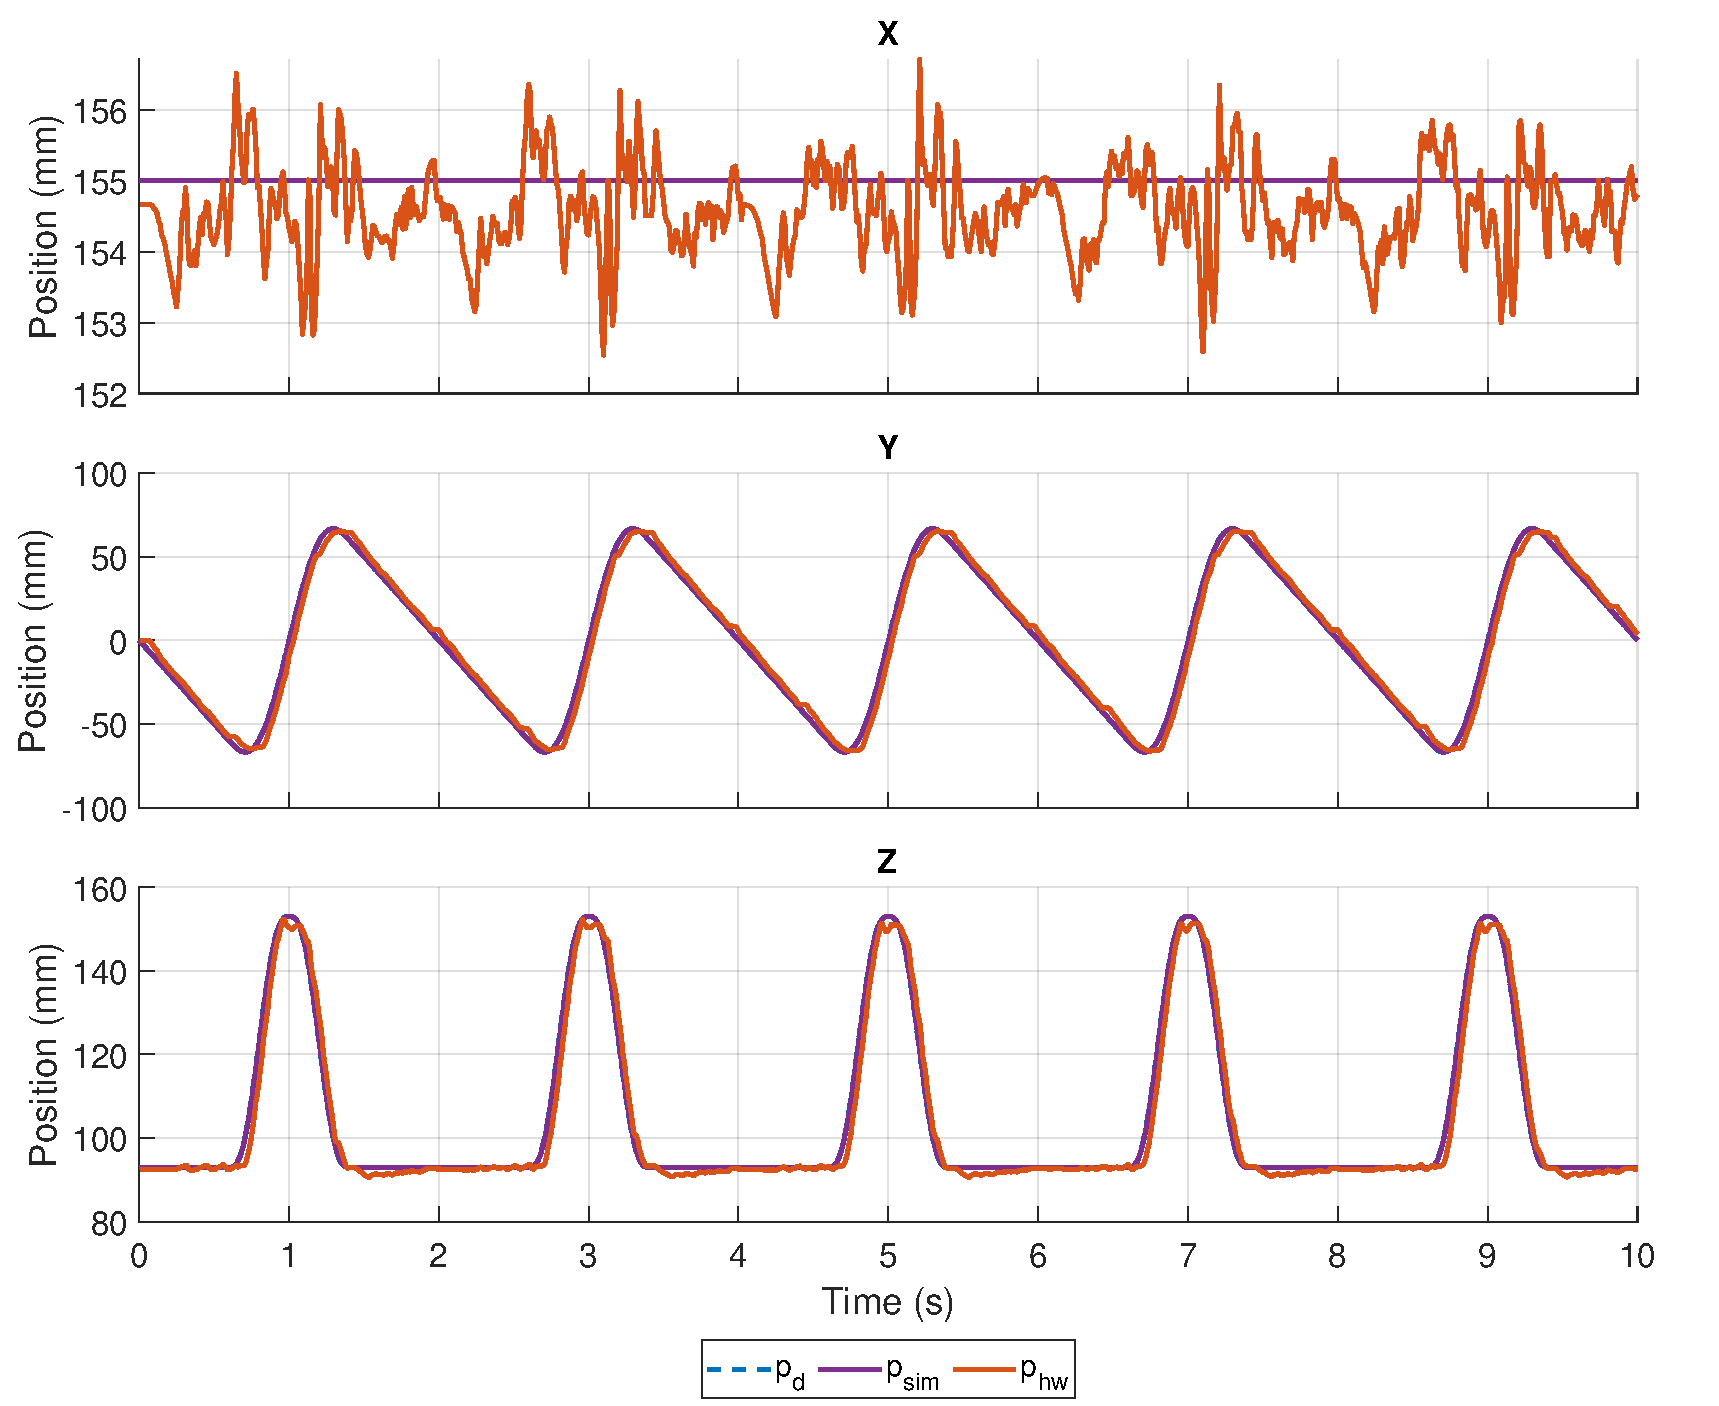
\includegraphics[width=\textwidth]{images2/cartesian_trajectories.pdf}
        \caption{Trajectory Tracking}
        \label{fig:cart_traj_exp}
    \end{subfigure}

    \begin{subfigure}[b]{0.8\textwidth}
        \centering
        
\includegraphics[width=\textwidth]{images2/cartesian_errors.pdf}
        \caption{Tracking Errors}
        \label{fig:cart_err_exp}
    \end{subfigure}
    \caption{Cartesian-Space Experiment Results.}
    \label{fig:cart_exp}
\end{figure}

The error plot (Figure \ref{fig:cart_err_exp}) reveals similarities in the simulation and experimental error shapes,
fundamentally changing only in amplitude (refer also to Figure \ref{fig:joint_results} for better understanding).
The amplitude difference can be attributed to a higher tracking delay, while the shape of the error is reasonably
due to inertial effects, purposely neglected at this stage of control.


\subsubsection{Joint Space Performance}

The performance at the actuator level is detailed in Figures \ref{fig:joint_traj_exp} and \ref{fig:joint_err_exp},
where once again it is visible how all three joints ($q_1, q_2, q_3$) track their respective references with
remarkable precision (also in this instance, the Simulation and Experimental plots differ by amplitude rather than
shape).

\begin{figure}[htbp]
    \centering
    \begin{subfigure}[b]{0.8\textwidth}
        \centering
        
\includegraphics[width=\textwidth]{images2/joint_trajectories.pdf}
        \caption{Trajectory Tracking}
        \label{fig:joint_traj_exp}
    \end{subfigure}

    \begin{subfigure}[b]{0.8\textwidth}
        \centering
        
\includegraphics[width=\textwidth]{images2/joint_errors.pdf}
        \caption{Tracking Errors}
        \label{fig:joint_err_exp}
    \end{subfigure}
    \caption{Joint-Space Experiment Results.}
    \label{fig:joint_exp}
\end{figure}


\subsubsection{Delay and Response Analysis}

To isolate the dynamic performance from the temporal evolution to promote a better visualization of the mentioned
tracking delay, Figure \ref{fig:tracking_delay_exp} presents the input-output correlation (Command vs. Measured
angle) for each joint. An ideal behaviour should be represented by a straight line ($y = x$), while a wider ellipse
would correspond to a higher tracking delay.

Both datasets populates the graph as expected (narrow ellipses for simulation and wider ellipses for the experiment).
Additionally, the slightly wider loops for $q_2$ and $q_3$ correlate with a higher inertial load due to gravity.

\begin{figure}[htbp]
    \centering
    \begin{subfigure}[b]{0.40\textwidth}
        \centering
        
\includegraphics[width=\textwidth]{images2/q_track_1.pdf}
        \caption{Hip ($q_1$)}
    \end{subfigure}
    \begin{subfigure}[b]{0.40\textwidth}
        \centering
        
\includegraphics[width=\textwidth]{images2/q_track_2.pdf}
        \caption{Knee ($q_2$)}
    \end{subfigure}

    \begin{subfigure}[b]{0.40\textwidth}
        \centering
        
\includegraphics[width=\textwidth]{images2/q_track_3.pdf}
        \caption{Ankle ($q_3$)}
    \end{subfigure}
    \caption{Tracking Delay Analysis.}
    \label{fig:tracking_delay_exp}
\end{figure}


\subsubsection{Quantitative Benchmark}

Unexpectedly, the tracking quality performs surprisingly well, despite the fact that the custom servomotor control
algorithm is originally designed for P2P control.

Ultimately, the tracking quality is quantified using the Root Mean Square Error (RMSE) metric (as per Section
\ref{sec:limitations}). Figure \ref{fig:rmse_benchmark} compares the simulation baseline against the physical
prototype.

While the experimental errors are naturally higher than the idealized simulation, the general trend matches for the
two cases, following similar magnitude patterns. The Cartesian RMSE is dominated by the Y-axis ($\approx 5.4$ mm),
consistent with the direction of maximum movement and backlash accumulation.
The main contributor to these errors in the experimental case, as shown in the previous section, was the tracking
delay. Nevertheless, the error remains however remarkably small for a low-cost prototype.

This quantitative benchmark conclusively validates the design approach: the custom actuators and the kinematic
model perform within the requirements defined at the outset of this thesis and well within acceptable limits for
stable locomotion.

\begin{figure}[htbp]
    \centering
    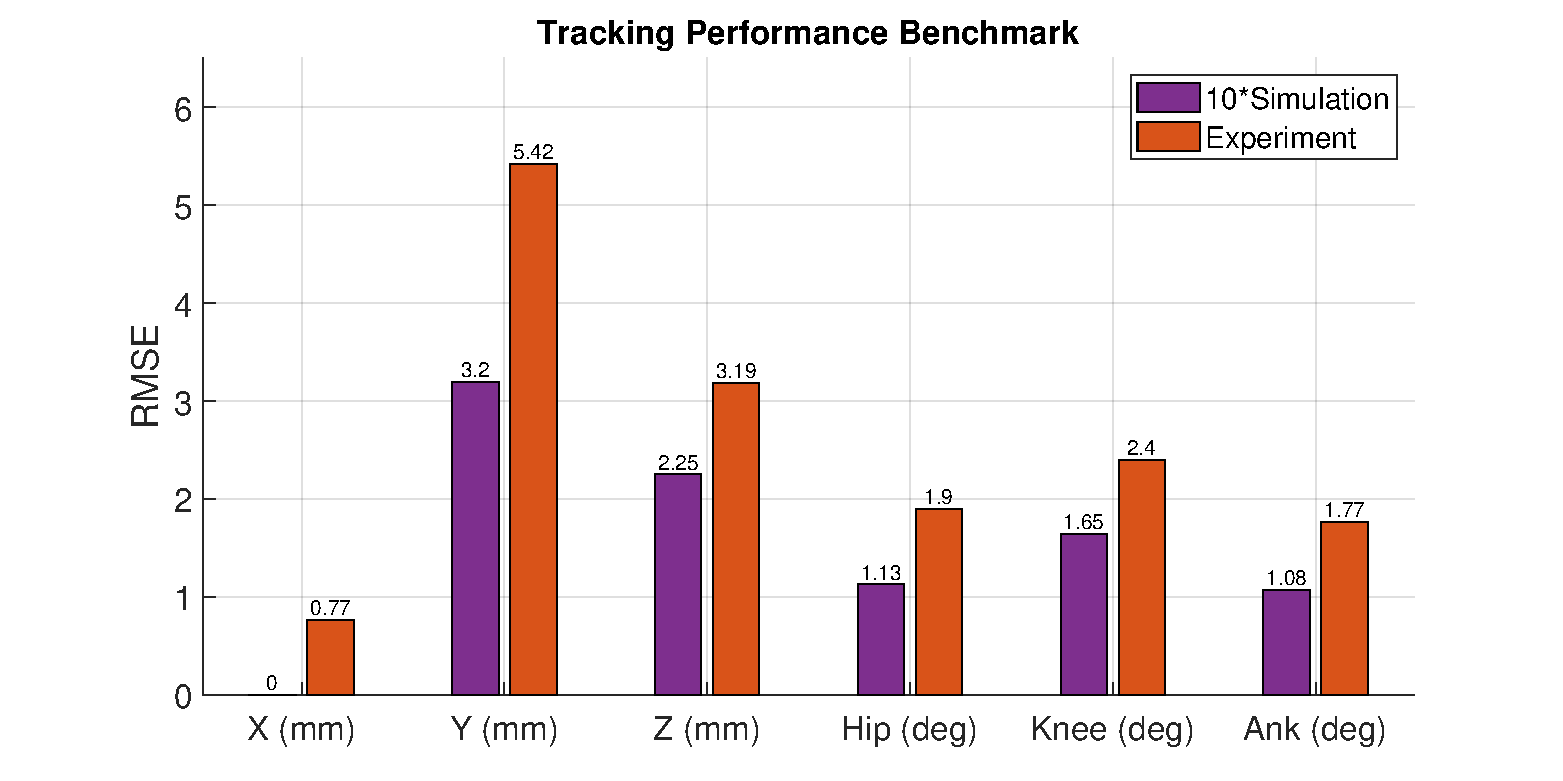
\includegraphics[width=0.98\textwidth]{images/rmse_benchmark.pdf}
    \caption{Simulation vs. Experiment Tracking Error.}
    \label{fig:rmse_benchmark}
\end{figure}